\documentclass[11pt]{article}

\usepackage[margin=1in]{geometry}
\usepackage{amsmath,amssymb,mathtools}
\usepackage{booktabs}
\usepackage{array}
\usepackage{graphicx}
\usepackage{hyperref}

\title{Continuum Reconstruction and Scalar-Transverse Coupling in Kernel-Induced Operator Systems}
\author{Tomislav Rupi\'c}
\date{March 2026}

\begin{document}
\maketitle

\begin{abstract}
The previous HAOS-IIP operator paper established that a Gaussian kernel substrate supports a low restricted transverse spectral band in addition to the scalar Laplacian branch. The present work tests two narrower numerical questions: whether that transverse band is consistent with a local continuum transverse operator, and how it responds to controlled scalar or kernel-geometry deformations. The committed Stage 3 and Stage 4 experiments show that the low restricted spectrum is consistent with a nearly gapless continuum transverse operator in the tested range and that smooth scalar deformations produce structured spectral response through stiffness renormalization, gap opening, and organized mode mixing. These results are presented strictly as operator-level numerical evidence; no claim is made for gauge dynamics, photons, or quantum field interpretation.
\end{abstract}

\section{Introduction}
The HAOS-IIP numerical program asks whether multiple continuum operator sectors can be reconstructed from a single kernel-defined discrete substrate. The first paper in the sequence, \emph{Kernel-Induced Operator Architecture and the Emergence of a Transverse Spectral Band on Discrete Substrates}, established two points: a Gaussian interaction kernel induces a scalar Laplacian limit, and after Hodge restriction the same substrate supports a descending transverse spectral band on periodic edge complexes. That paper did not address what continuum operator the band approximates or how it responds to controlled changes in the underlying scalar or kernel geometry.

This follow-up paper addresses those two questions using only the committed Stage 3 and Stage 4 experiments already present in the repository. The operator architecture is frozen throughout: the kernel, graph construction, scalar branch, edge Hodge operator, and restricted transverse subspace are inherited unchanged from the earlier work.

The Stage 3 results provide four diagnostics of continuum behavior. The low restricted spectrum follows the continuum transverse ordering on a periodic box, a minimal fit of the form $\lambda_k \approx c_{\mathrm{eff}} |q_k|^2 + m_{\mathrm{eff}}$ yields a stable stiffness and numerically vanishing gap, real-space correlations remain extended with modest anisotropy, and coarse-grained reconstruction produces decreasing residuals for $\nabla \times \nabla \times A \approx \lambda A$ while the divergence stays at machine precision.

The Stage 4 results test how the same restricted transverse band responds to controlled scalar or kernel-geometry deformation. Smooth radial, anisotropic, and localized-bump deformations shift the low spectrum, mix the low modes in a structured way, reduce the fitted stiffness, and open a finite gap in the tested deformed fits. The purpose of the paper is narrow: it documents operator-level numerical evidence for continuum reconstruction and structured scalar-transverse coupling, without introducing new dynamical claims.

\section{Frozen Operator Architecture}
\begin{align}
A_{ij} &= \exp\!\left(-\frac{|x_i-x_j|^2}{2\varepsilon_k}\right),\\
L_0 &= D - A,\\
L_1 &= d_0 d_0^* + d_1^* d_1,\\
T &= d_1^* d_1\big|_{\ker(d_0^*) \cap (\mathcal{H}^1)^\perp}.
\end{align}
These operators are inherited without change from the first paper. The kernel, graph construction, normalization, edge weights, and restricted subspace are all frozen for the present study. The only new ingredients in Stages 3 and 4 are the diagnostics used to characterize the low restricted transverse spectrum and the controlled scalar or embedding deformations used to test its response.

\section{Restricted Transverse Sector}
\begin{equation}
C^1 = \operatorname{im} d_0 \oplus \mathcal{H}^1 \oplus \operatorname{im} d_1^*.
\end{equation}
The unrestricted edge spectrum mixes exact gradient modes and harmonic torus cycles into its lowest levels, so it is not the right object for testing a transverse continuum branch. The operator examined here is the restriction of $d_1^* d_1$ to $\ker(d_0^*) \cap (\mathcal{H}^1)^\perp$, which removes both exact leakage and harmonic modes. All Stage 3 and Stage 4 results below therefore refer to the same restricted coexact branch, with the repository continuing to record restricted eigenvalues together with divergence norm, curl norm, and inverse participation ratio.
All numerical datasets cited below correspond to stamped artifacts in the public repository, and each figure references the timestamped output from which it was drawn.

\section{Continuum Spectral Comparison}
All numerical statements in this section correspond to stamped Stage 3 artifacts committed in the public repository. The first diagnostic compares the low restricted transverse spectrum against the continuum transverse mode ordering on a periodic box generated from nonzero integer wavevectors with transverse multiplicity two.

The main result is that the low restricted modes follow the continuum ordering and spacing pattern across the tested branches. In the baseline branch, the first-ten relative spectrum error is $0.2189$ at each of $n=12,16,20$, while the first-ten spacing error is numerically zero in the implemented comparison metric. The mild-defect branches are at least as consistent with the continuum ordering: at $n=20$ the first-ten relative spectrum error is $0.0131$ for the puncture branch, $0.0430$ for the line-defect branch, and $0.1647$ for the flux-tube branch.

The bounded interpretation is that the low restricted spectrum is organized like the low branch of a continuum transverse operator in the tested range. This comparison does not establish dynamics. It shows only that the low-band ordering and low-mode spacing match the continuum reference structure at the operator level.
\begin{figure}[t]
\centering
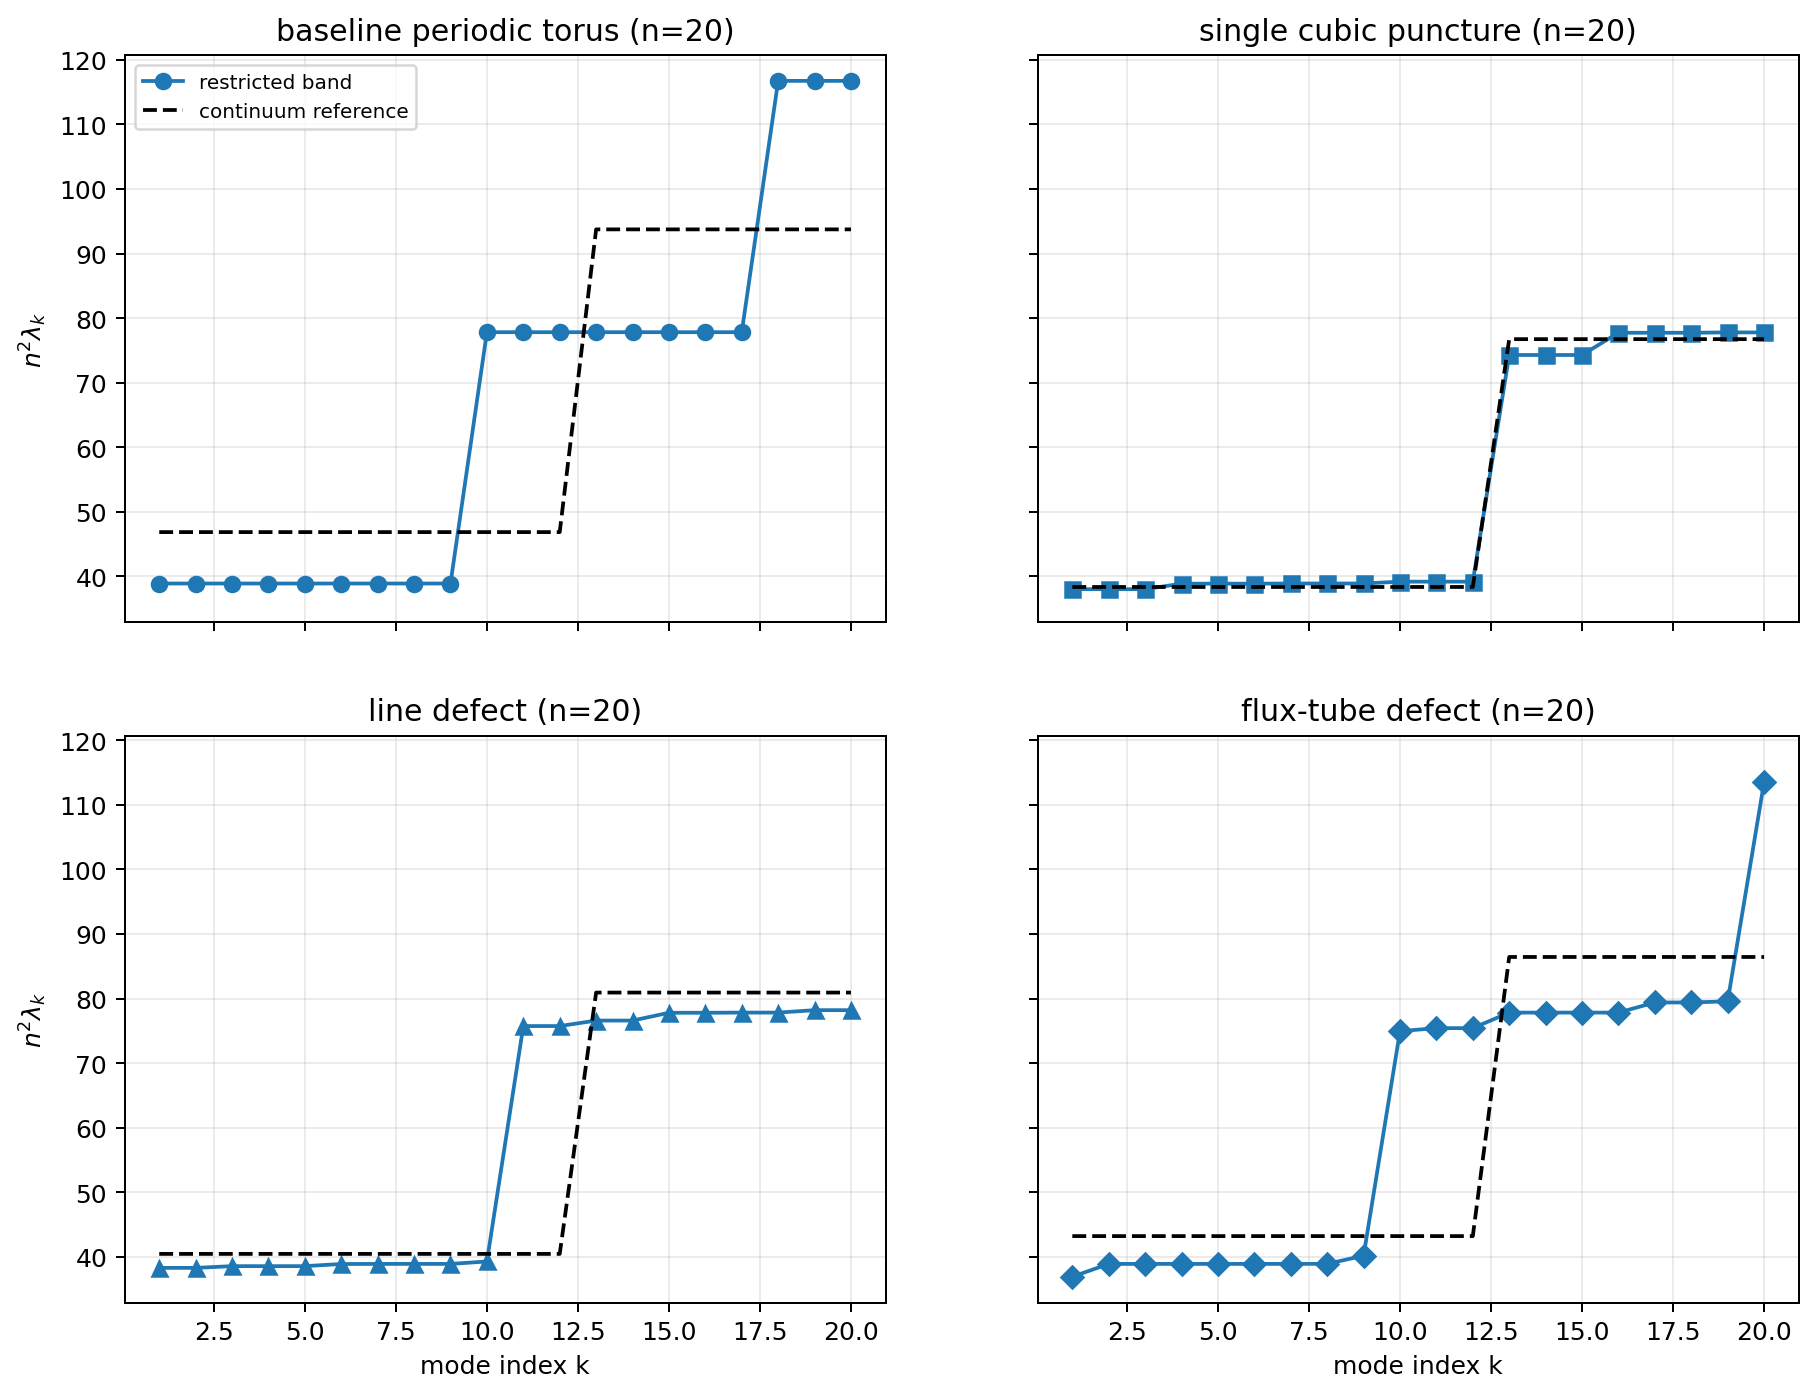
\includegraphics[width=0.48\linewidth]{../plots/20260310_150006_transverse_continuum_comparison.png}
\hfill
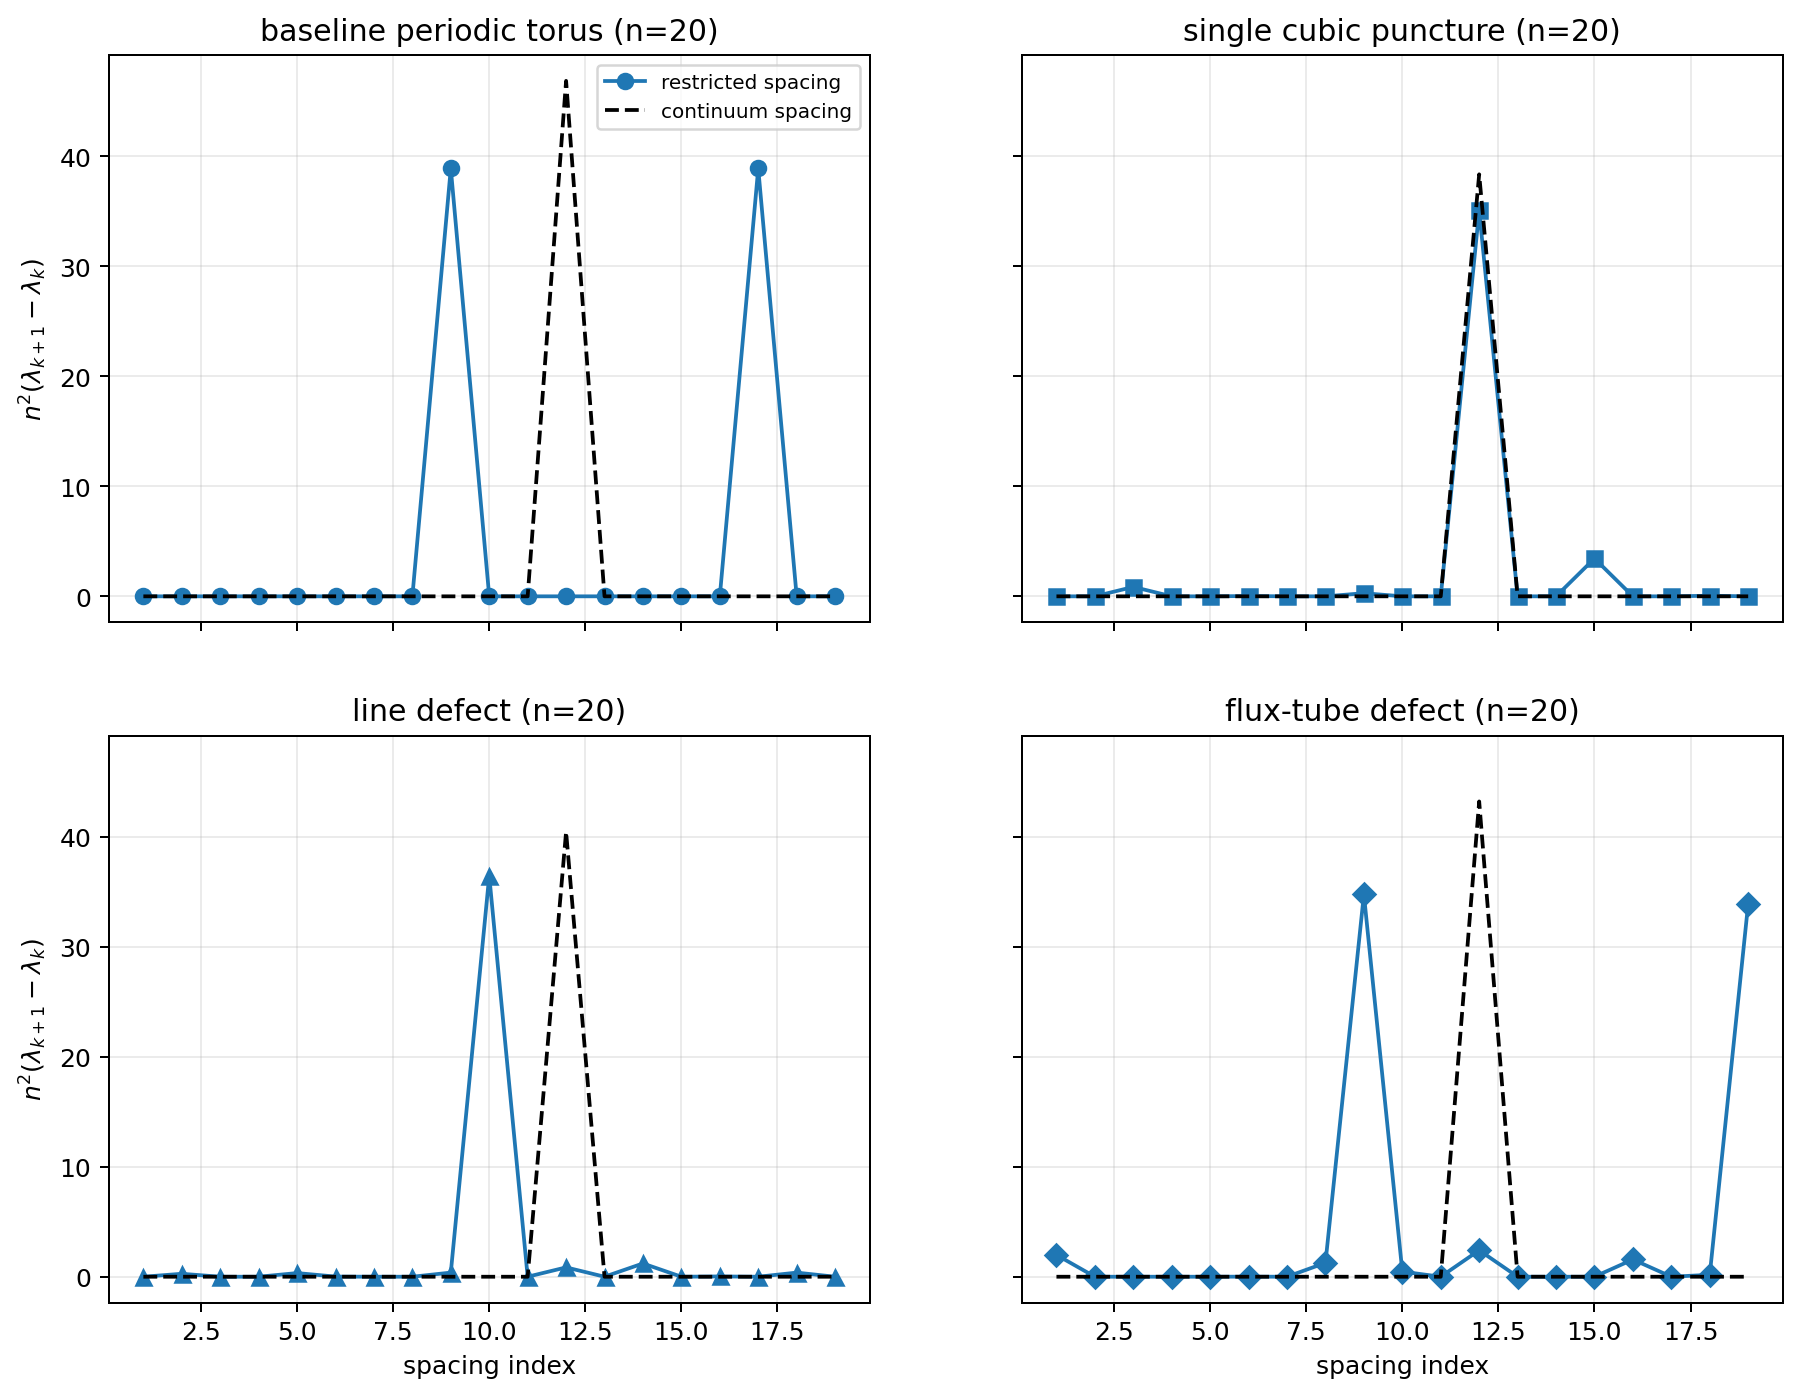
\includegraphics[width=0.48\linewidth]{../plots/20260310_150006_transverse_mode_spacing.png}
\caption{Stage 3 continuum comparison for the restricted transverse band. Left: low eigenvalues compared with the continuum transverse ordering on the periodic box. Right: low-mode spacing comparison for the same stamped run.}
\label{fig:continuum-comparison}
\end{figure}

\section{Effective Operator Fit}
\begin{equation}
\lambda_k \approx c_{\mathrm{eff}} |q_k|^2 + m_{\mathrm{eff}}.
\end{equation}
This minimal fit is applied to the distinct low spectral families on the clean periodic branch for $n=12,16,20,24$. The fitted stiffness is nearly stable,
\begin{equation}
c_{\mathrm{eff}} = 37.9206,\ 38.5949,\ 38.9108,\ 39.0834,
\end{equation}
while the fitted gap remains numerically zero within floating-point resolution,
\begin{equation}
m_{\mathrm{eff}} = -8.3\times 10^{-17},\ -2.5\times 10^{-16},\ -2.1\times 10^{-17},\ 0,
\end{equation}
with $R^2 = 1.00000$ in each fitted case.

The direct numerical reading is that the low restricted branch is consistent with a nearly gapless continuum operator with stable stiffness in the tested range. The fit is intentionally minimal and is used only to summarize the low-band structure, not to introduce new field content.
\begin{figure}[t]
\centering
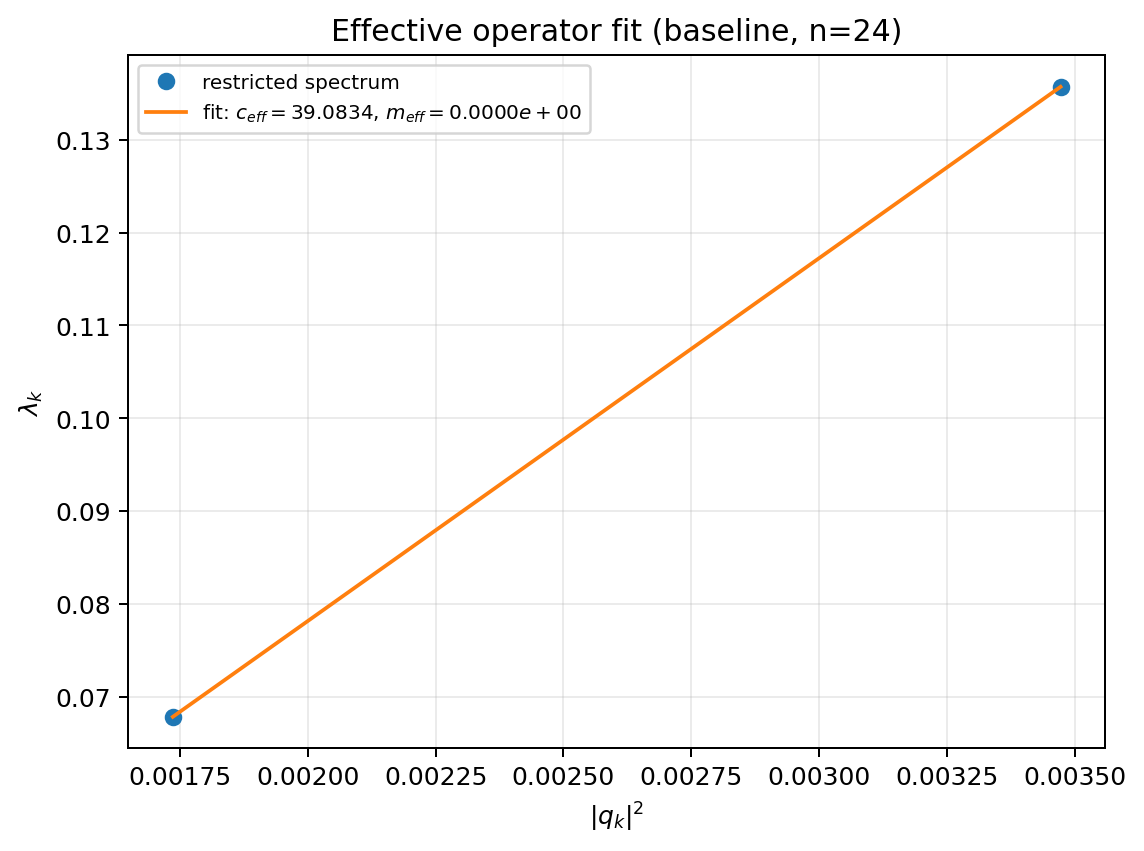
\includegraphics[width=0.32\linewidth]{../plots/20260310_155713_effective_operator_fit.png}
\hfill
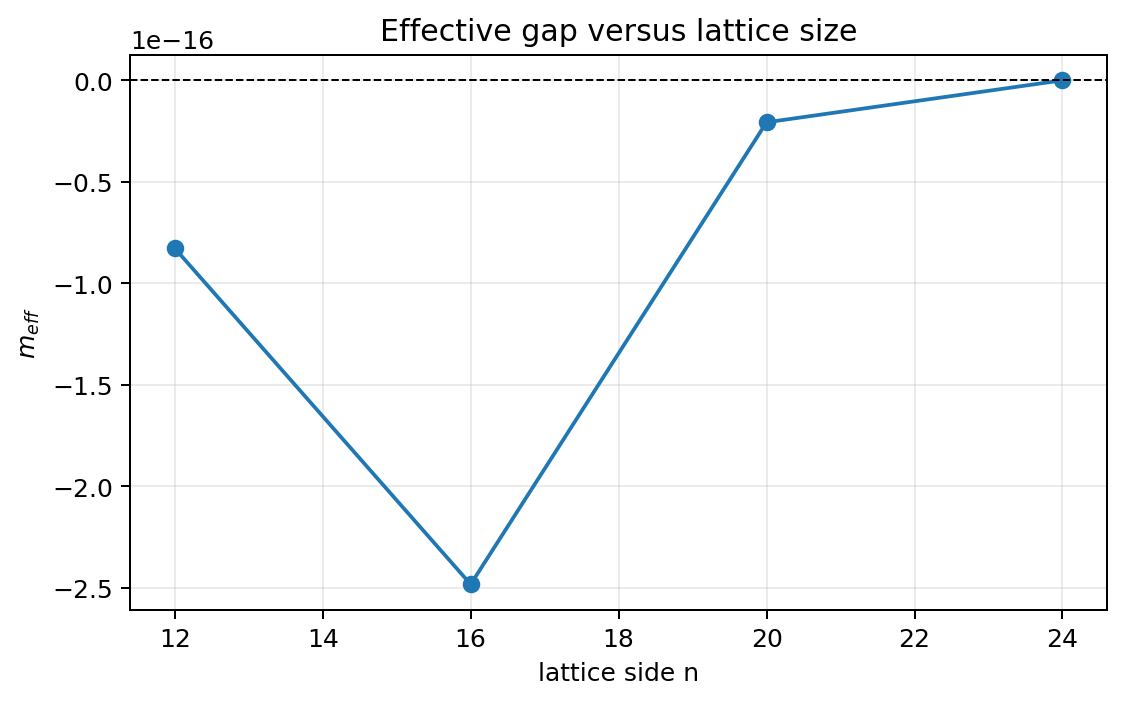
\includegraphics[width=0.32\linewidth]{../plots/20260310_155713_effective_gap_vs_n.png}
\hfill
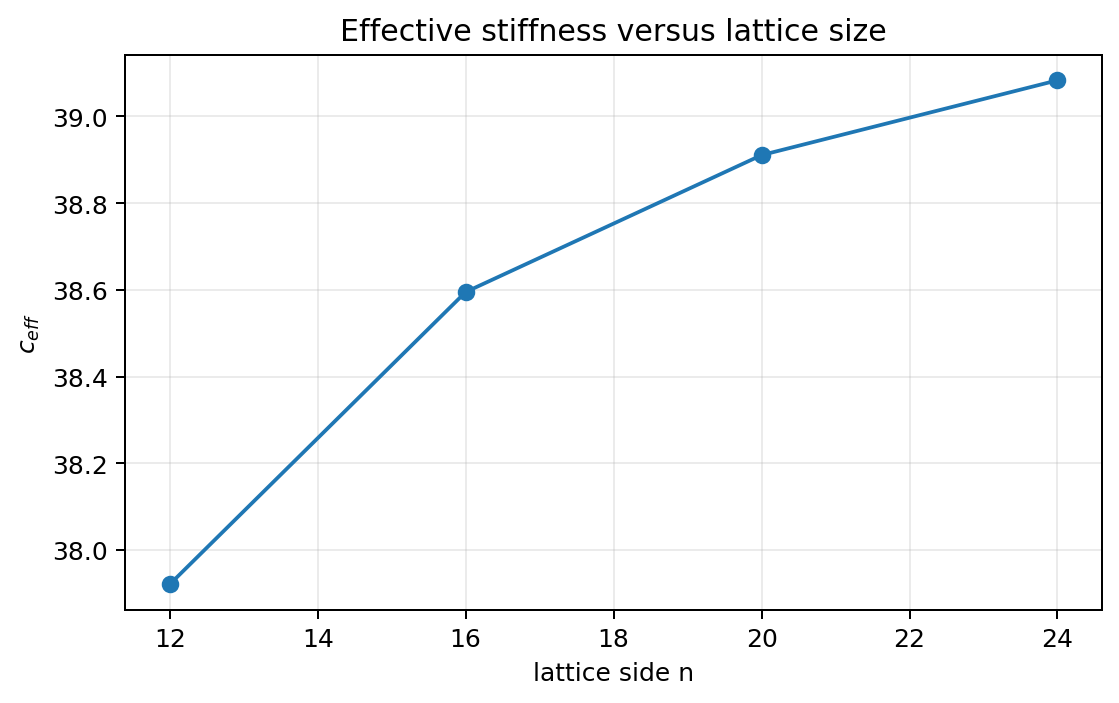
\includegraphics[width=0.32\linewidth]{../plots/20260310_155713_effective_stiffness_vs_n.png}
\caption{Stage 3 effective-operator fit on the clean periodic branch. Left: low-band fit to $\lambda_k \approx c_{\mathrm{eff}} |q_k|^2 + m_{\mathrm{eff}}$. Center and right: fitted gap and stiffness across the tested lattice sizes.}
\label{fig:effective-fit}
\end{figure}

\section{Real-Space Continuum Diagnostics}
The remaining Stage 3 diagnostics test whether the low restricted modes behave like extended continuum fields in real space. The two-point correlation experiment shows a correlation-length proxy of $0.0940$ at $n=12$ and $0.0884$ at $n=16$, while the anisotropy ratio drops from $4.61$ to $1.20$. Over the same range, the lowest-mode inverse participation ratio decreases from $5.31\times 10^{-4}$ to $1.16\times 10^{-4}$.

The coarse-grained PDE reconstruction then tests whether the same low modes satisfy a local relation of the form
\begin{equation}
\nabla \times \nabla \times A \approx \lambda A,
\qquad
\nabla \cdot A \approx 0.
\end{equation}
For the lowest reconstructed mode, the relative curl-curl residual decreases from $0.050648$ at $n=12$ to $0.028620$ at $n=16$, while the relative divergence norm remains at machine precision.

Taken together, these diagnostics support a narrow conclusion: the low restricted modes are extended, become more isotropic at the larger tested size, and approximately satisfy a local coarse-grained PDE. This is the strongest real-space statement supported by the Stage 3 data.
\begin{figure}[t]
\centering
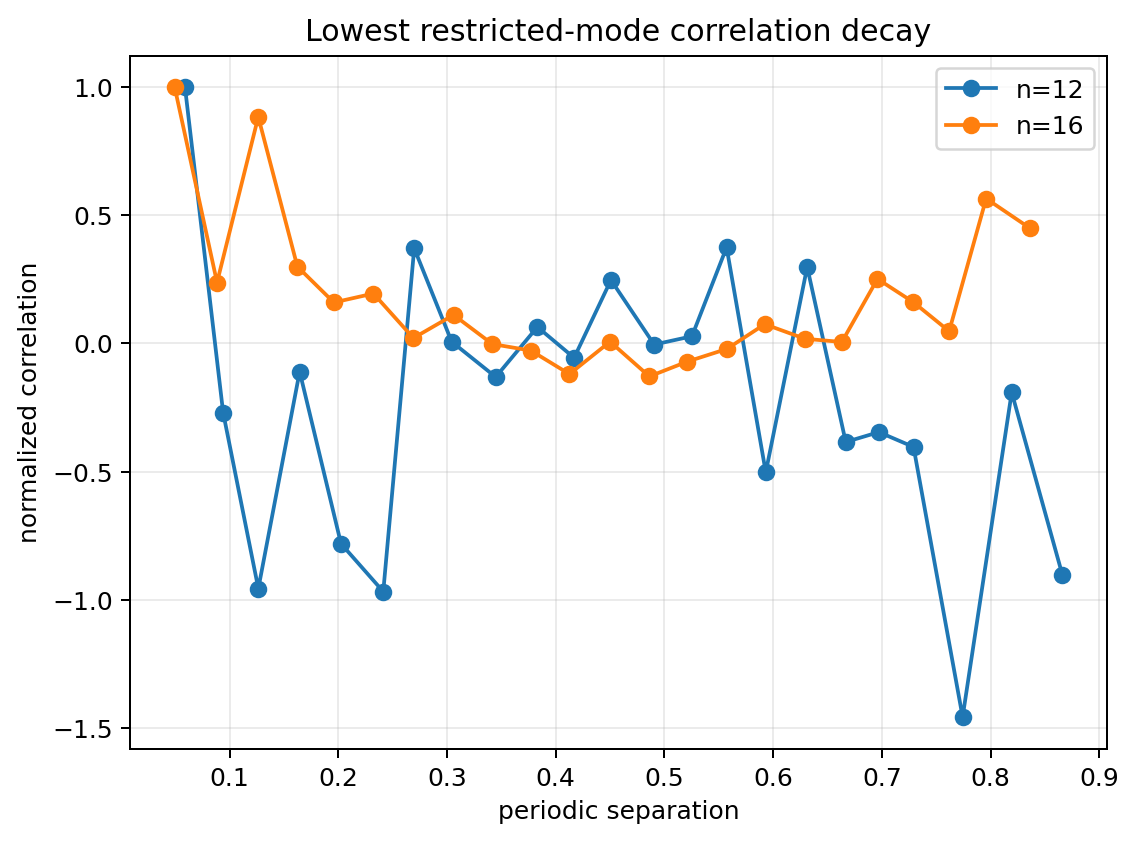
\includegraphics[width=0.48\linewidth]{../plots/20260310_155153_transverse_correlation_decay.png}
\hfill
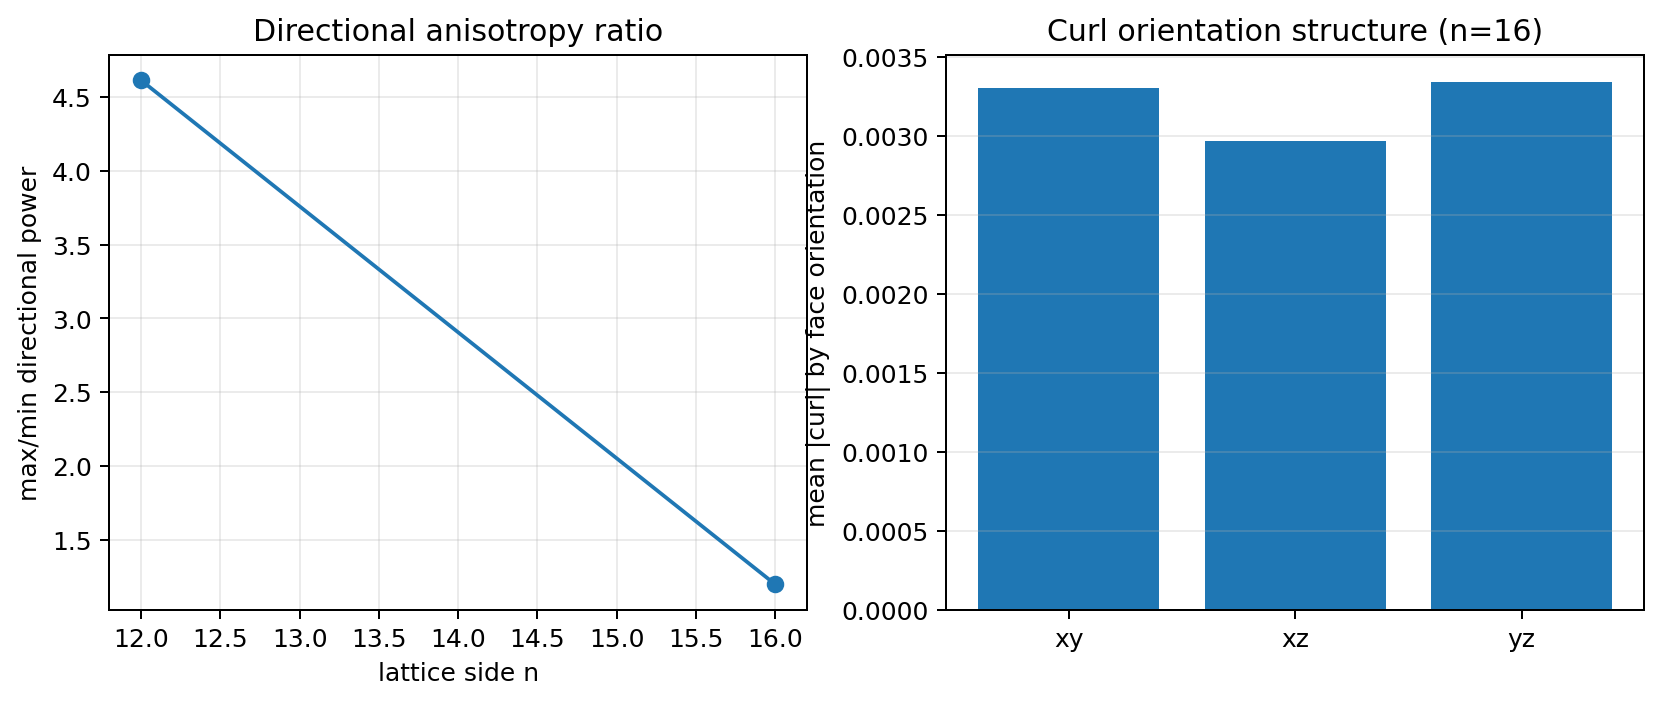
\includegraphics[width=0.48\linewidth]{../plots/20260310_155153_transverse_anisotropy.png}
\caption{Stage 3 real-space correlation diagnostics for the lowest restricted transverse mode. Left: correlation decay. Right: anisotropy summary across the tested sizes.}
\label{fig:correlations}
\end{figure}

\begin{figure}[t]
\centering
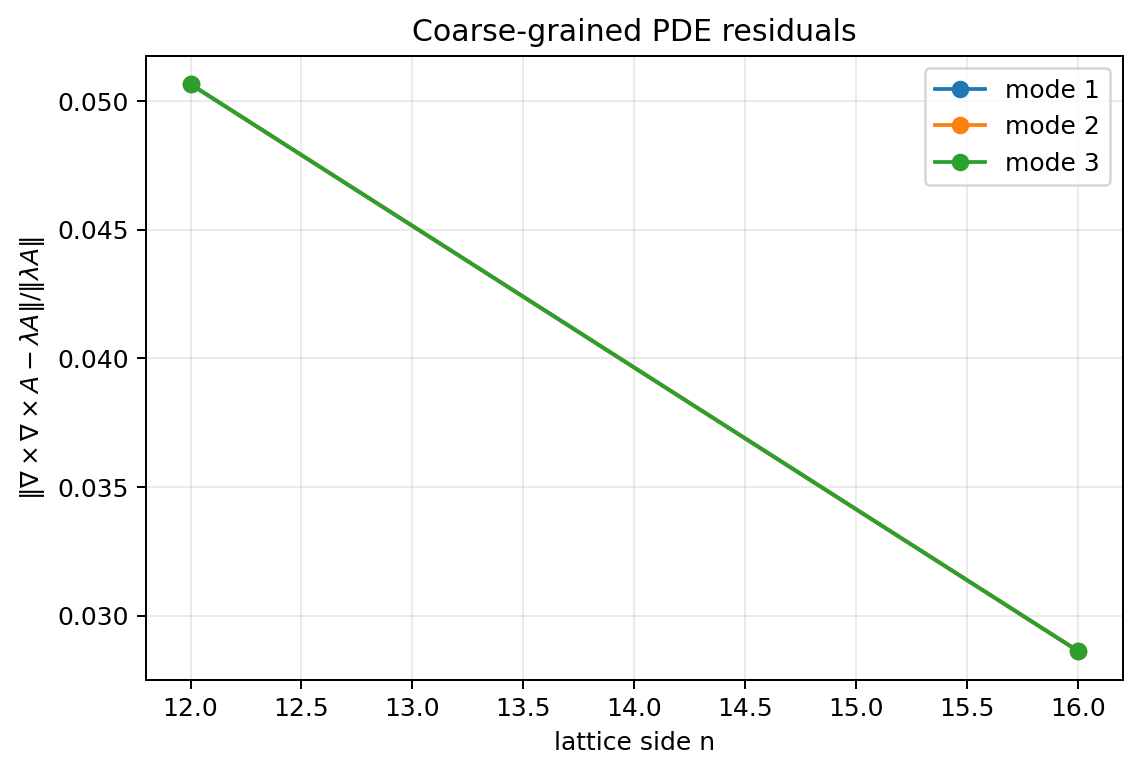
\includegraphics[width=0.48\linewidth]{../plots/20260310_154831_pde_reconstruction_residuals.png}
\hfill
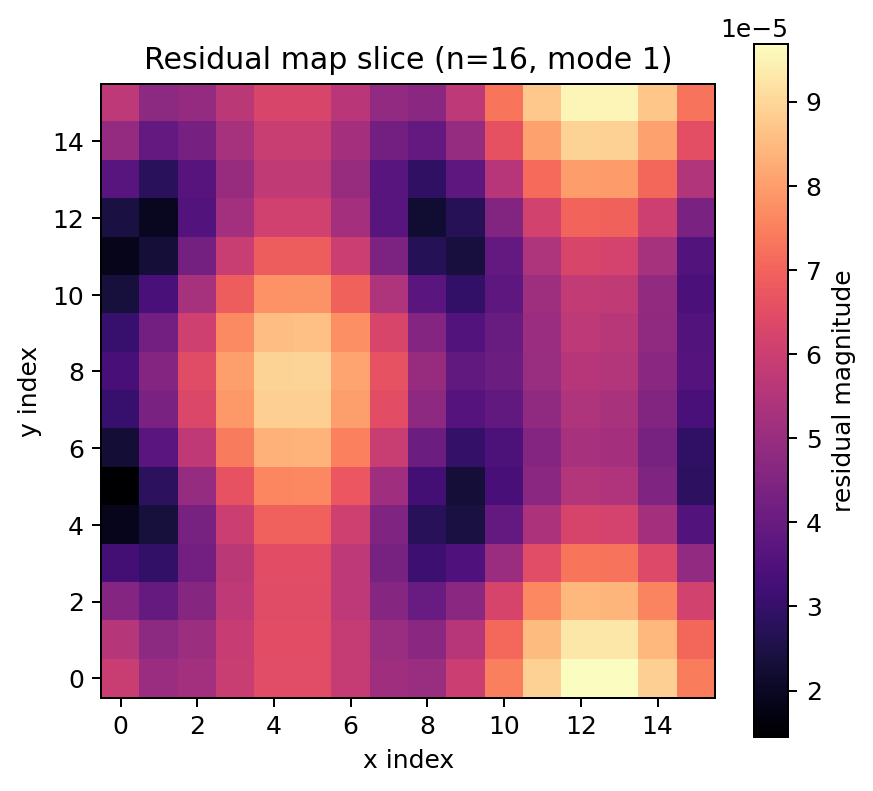
\includegraphics[width=0.48\linewidth]{../plots/20260310_154831_transverse_field_residual_maps.png}
\caption{Stage 3 coarse-grained PDE reconstruction. Left: residual of $\nabla \times \nabla \times A \approx \lambda A$ across lattice size. Right: representative residual maps for the reconstructed low modes.}
\label{fig:pde-reconstruction}
\end{figure}

\section{Scalar-Transverse Deformation Response}
Stage 4 asks whether the low restricted transverse band responds coherently when the scalar or kernel geometry is deformed while the operator definitions remain fixed. Three deformation families are used at amplitudes $\eta = 0.02, 0.05, 0.10$: a smooth radial deformation of the embedding, an anisotropic box deformation, and a localized scalar bump. These are evaluated on the baseline, puncture, and line-defect branches at $n=12$.

The main observation is that the low restricted spectrum shifts smoothly under all tested deformations while the matched low-mode overlaps remain moderate to high depending on branch and deformation family. For the baseline anisotropic case at $\eta=0.10$, the lowest restricted eigenvalue shifts by
\begin{equation}
\Delta \lambda_1 = -4.79 \times 10^{-4},
\end{equation}
with mean matched overlap $0.4121$. The corresponding overlaps are higher on the defected branches, reaching $0.8125$ for the puncture anisotropic case and $0.7297$ for the line-defect anisotropic case at the same amplitude. The bump family produces smaller spectral shifts than the radial and anisotropic families.

The bounded interpretation is that the transverse band deforms smoothly and repeatably under scalar or embedding changes. The response is small in absolute magnitude but systematic across amplitudes and branches.
\begin{figure}[t]
\centering
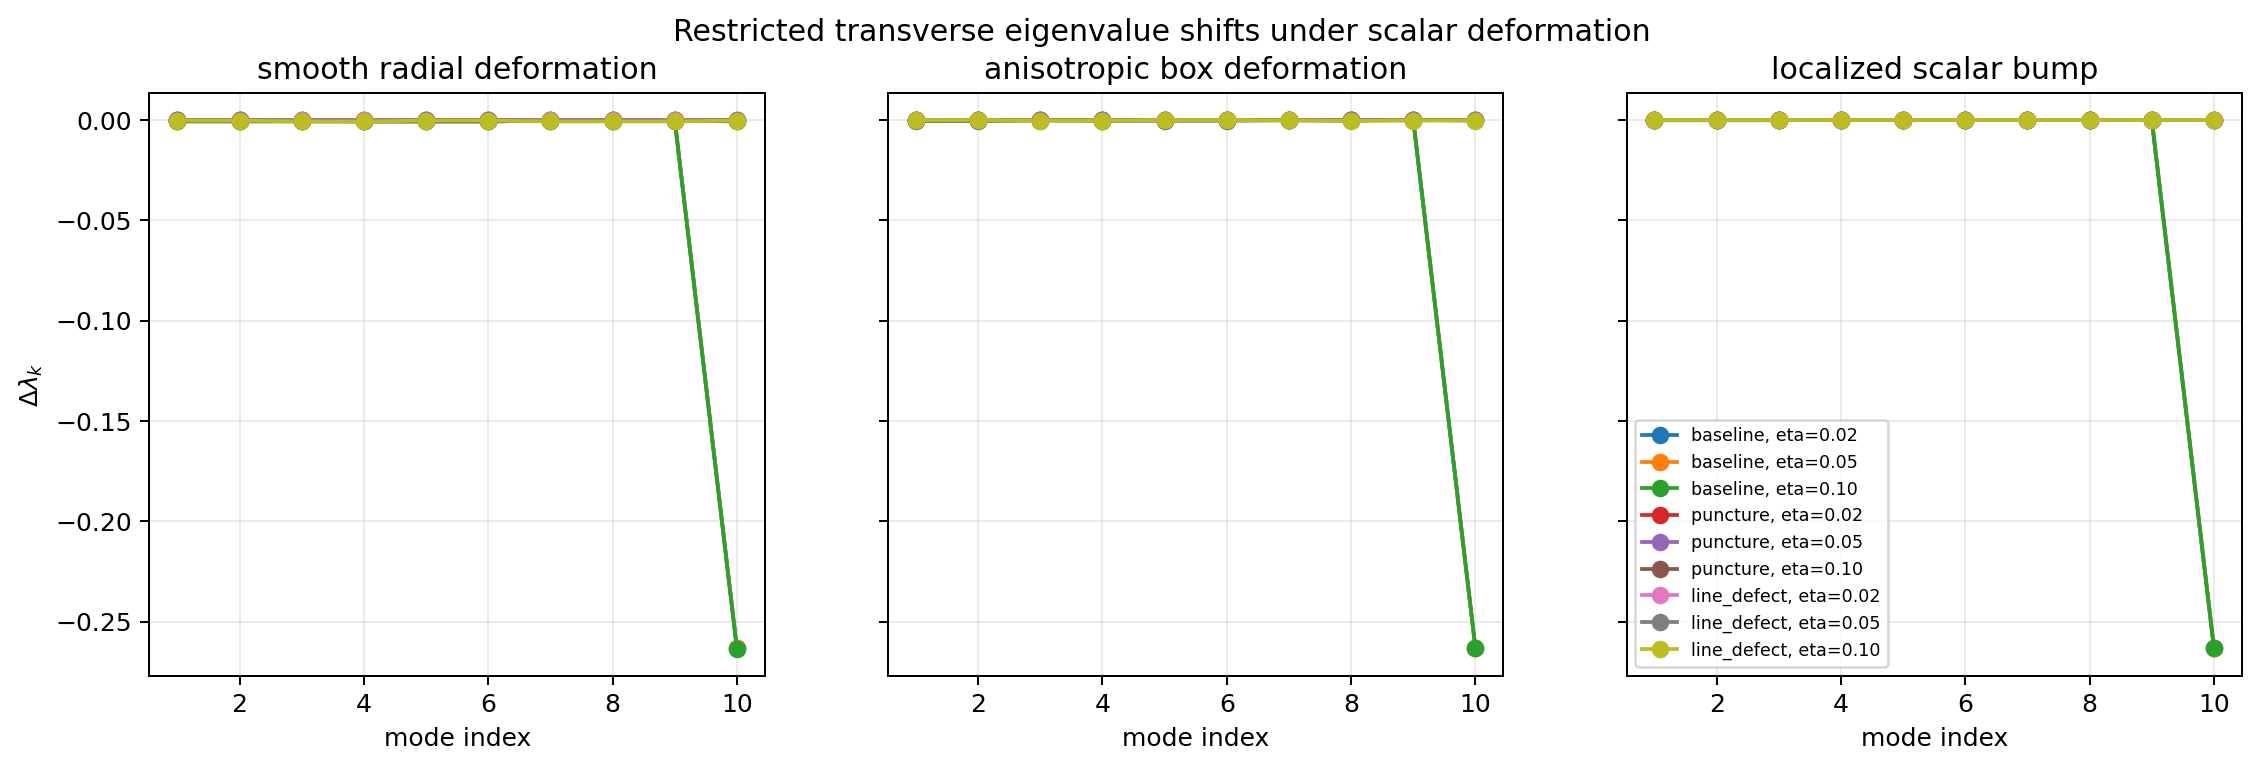
\includegraphics[width=0.32\linewidth]{../plots/20260310_164041_scalar_transverse_eigenvalue_shifts.png}
\hfill
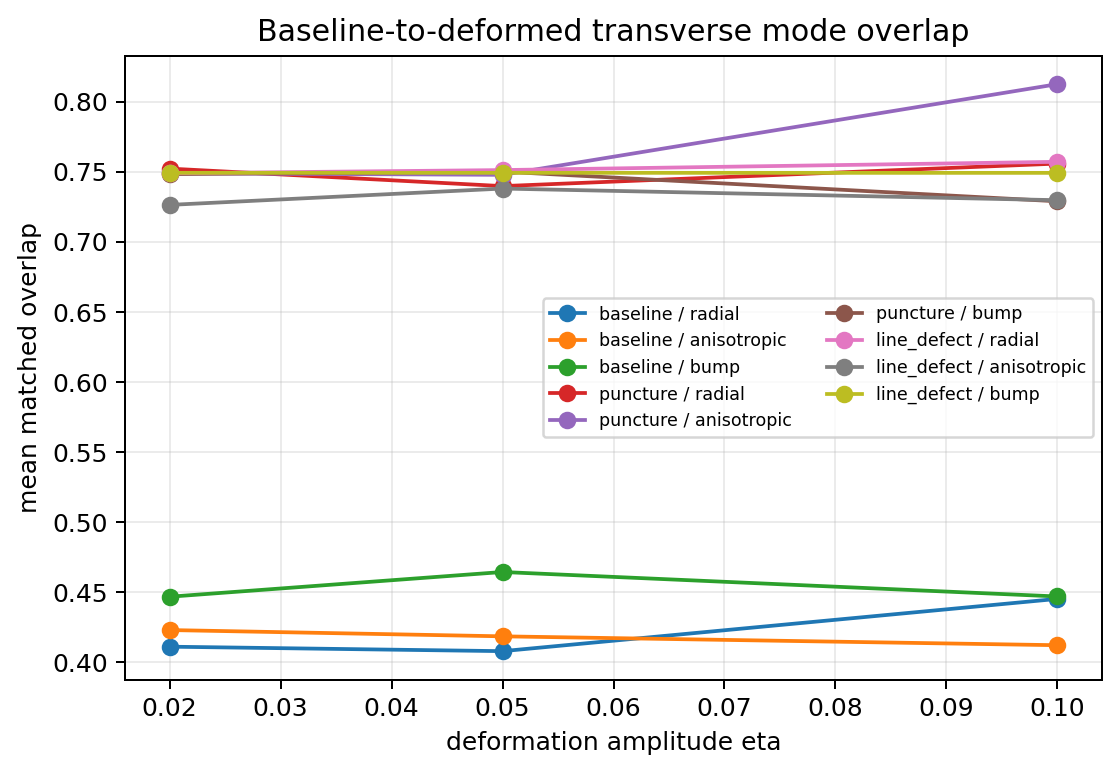
\includegraphics[width=0.32\linewidth]{../plots/20260310_164041_scalar_transverse_mode_overlap.png}
\hfill
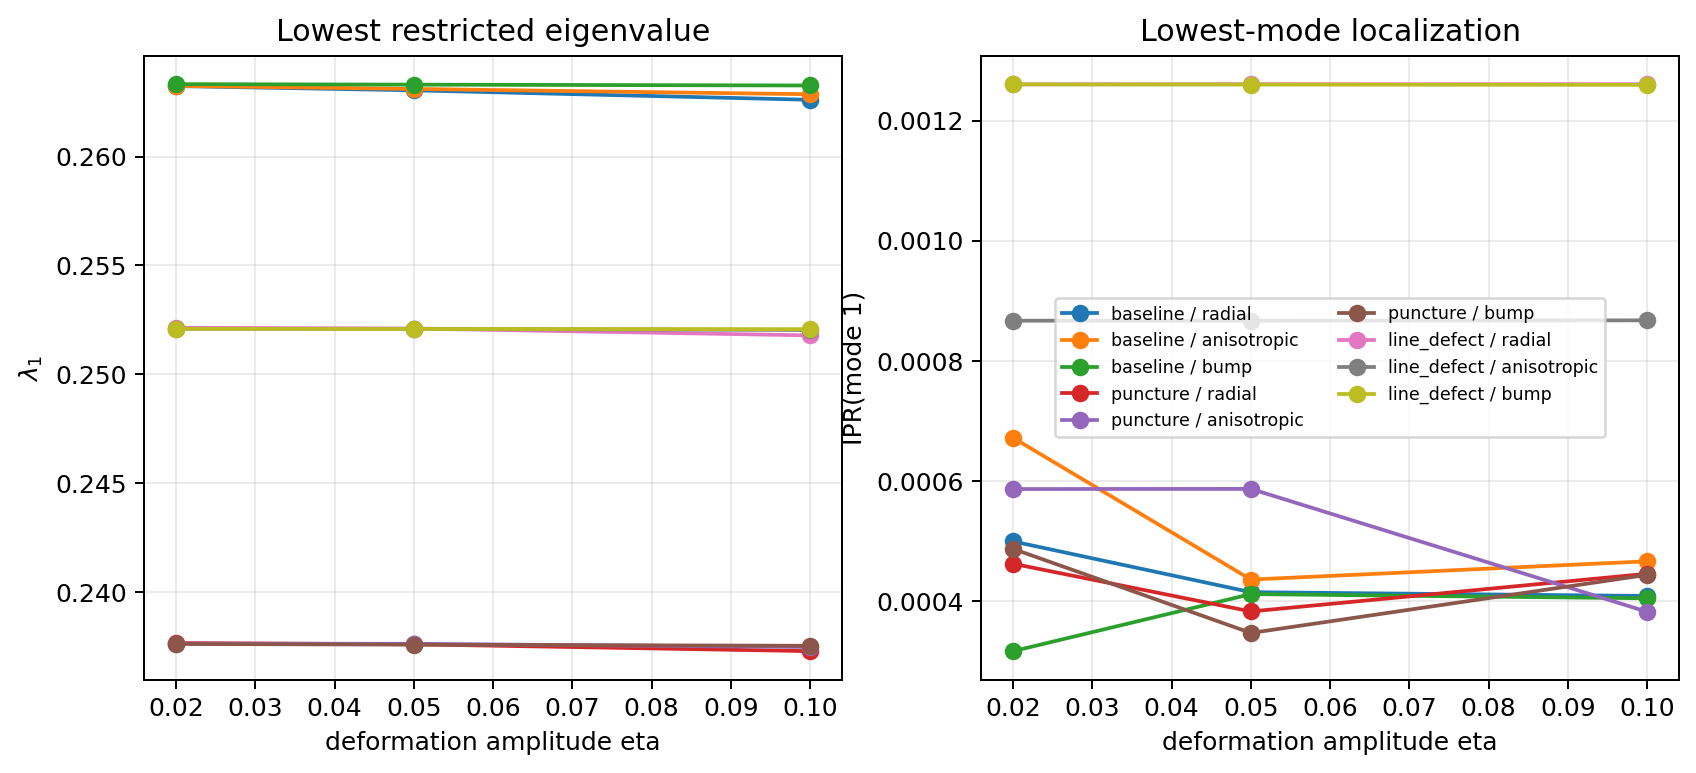
\includegraphics[width=0.32\linewidth]{../plots/20260310_164041_scalar_transverse_deformation_response.png}
\caption{Stage 4 deformation-response diagnostics for the low restricted transverse band under radial, anisotropic, and localized-bump deformations with $\eta=0.02,0.05,0.10$.}
\label{fig:deformation-response}
\end{figure}

\section{Coupling Structure and Effective Parameters}
The coupling-matrix experiment measures the low-mode response
\begin{equation}
C_{ij}(\eta) = \langle a_i, (T_\eta - T_0)a_j \rangle
\end{equation}
for the baseline anisotropic deformation. Its weight remains structured but is not diagonal-dominant. The diagonal fraction rises from $0.0738$ at $\eta=0.02$ to $0.3365$ at $\eta=0.10$, while the off-diagonal fraction remains larger than the diagonal contribution throughout the tested range. The resulting mode mixing is therefore organized inside the low-mode block rather than purely diagonal or random.

The same deformation data were then fit back to the effective form $\lambda_k \approx c_{\mathrm{eff}} |q_k|^2 + m_{\mathrm{eff}}$. In the committed Stage 4 fit, all three deformation families at $n=12$ reduce the effective stiffness from the undeformed value $c_{\mathrm{eff}}=37.9206$ to approximately $23.6$ at $\eta=0.10$, while opening a finite gap of order $m_{\mathrm{eff}} \approx 9.88\times 10^{-2}$. For example, the anisotropic family at $\eta=0.10$ gives
\begin{equation}
c_{\mathrm{eff}} = 23.6545,
\qquad
m_{\mathrm{eff}} = 9.8846 \times 10^{-2}.
\end{equation}
Within the tested range, scalar deformation therefore acts as a combined stiffness reduction and gap-opening perturbation on the low transverse band.

The backreaction maps show that this response is spatially structured rather than uniform. For the baseline bump at $\eta=0.10$, the mean sensitivity is $0.008907$ and the correlation with the bump profile is $-0.0934$, so the response is not simply proportional to the scalar perturbation itself. In the puncture branch at the same amplitude, the mean sensitivity is $0.005312$ with profile correlation $0.2862$, again indicating nontrivial spatial structure rather than a flat redistribution of amplitude.
\begin{figure}[t]
\centering
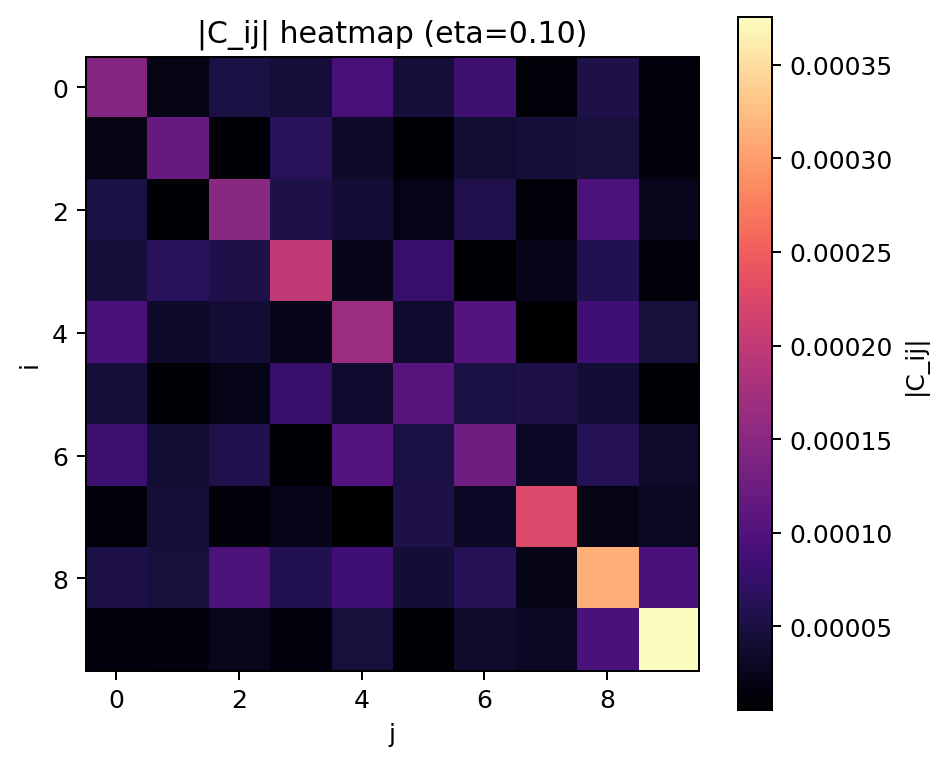
\includegraphics[width=0.48\linewidth]{../plots/20260310_164216_transverse_coupling_matrix_heatmap.png}
\hfill
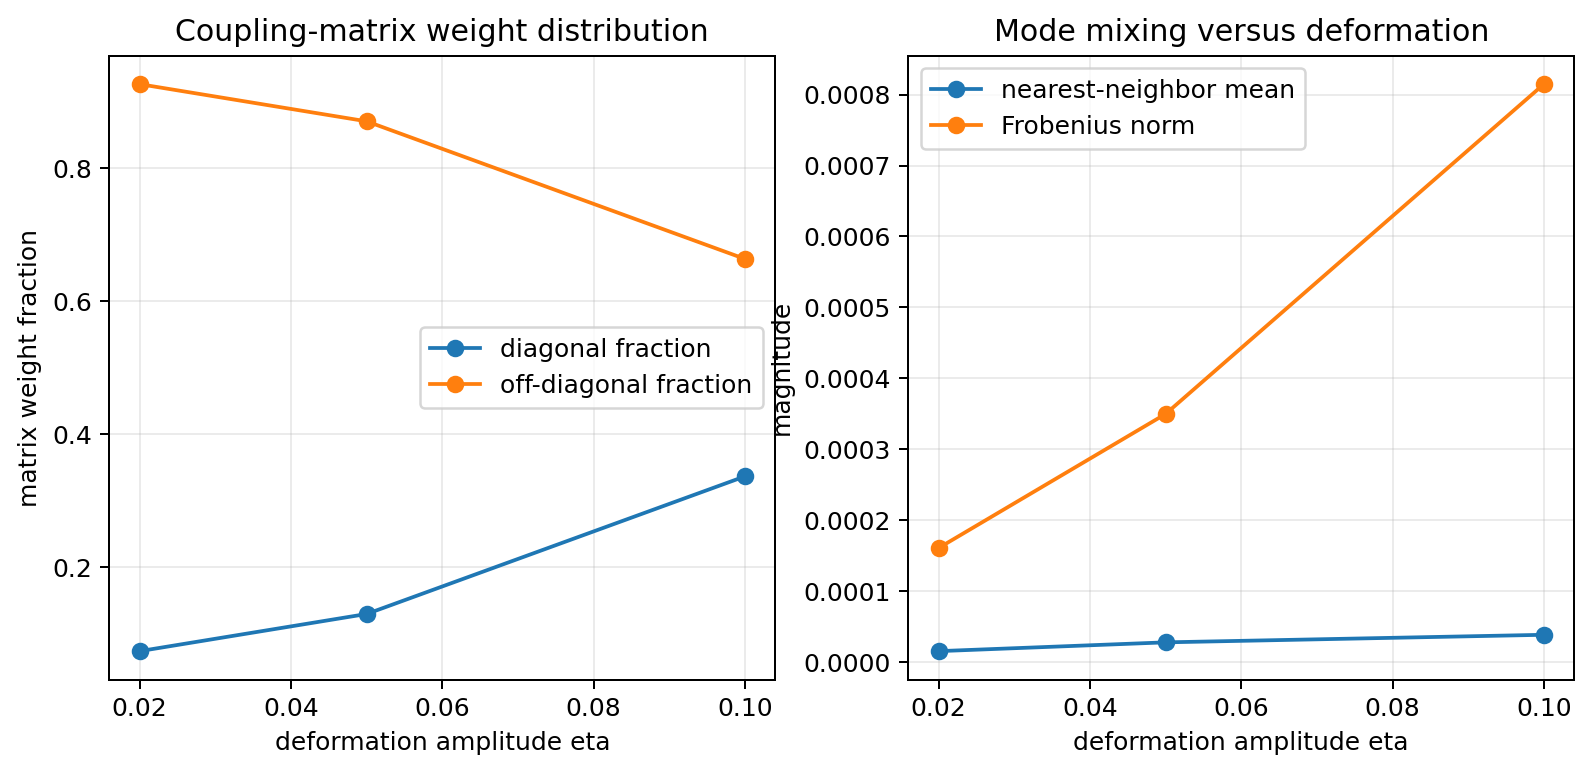
\includegraphics[width=0.48\linewidth]{../plots/20260310_164216_transverse_mode_mixing_vs_eta.png}
\caption{Stage 4 coupling-matrix diagnostics for the baseline anisotropic deformation. Left: low-mode coupling matrix heatmap. Right: mode-mixing summary versus deformation amplitude.}
\label{fig:coupling-matrix}
\end{figure}

\begin{figure}[t]
\centering
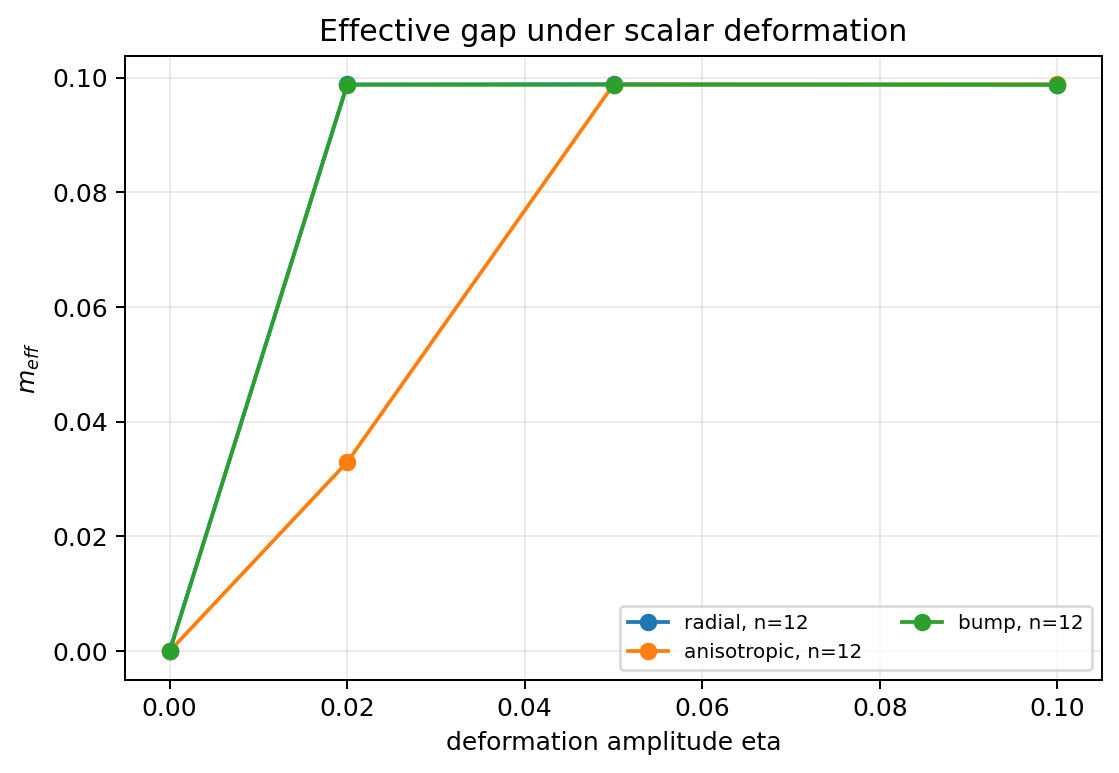
\includegraphics[width=0.48\linewidth]{../plots/20260310_164600_transverse_gap_vs_deformation.png}
\hfill
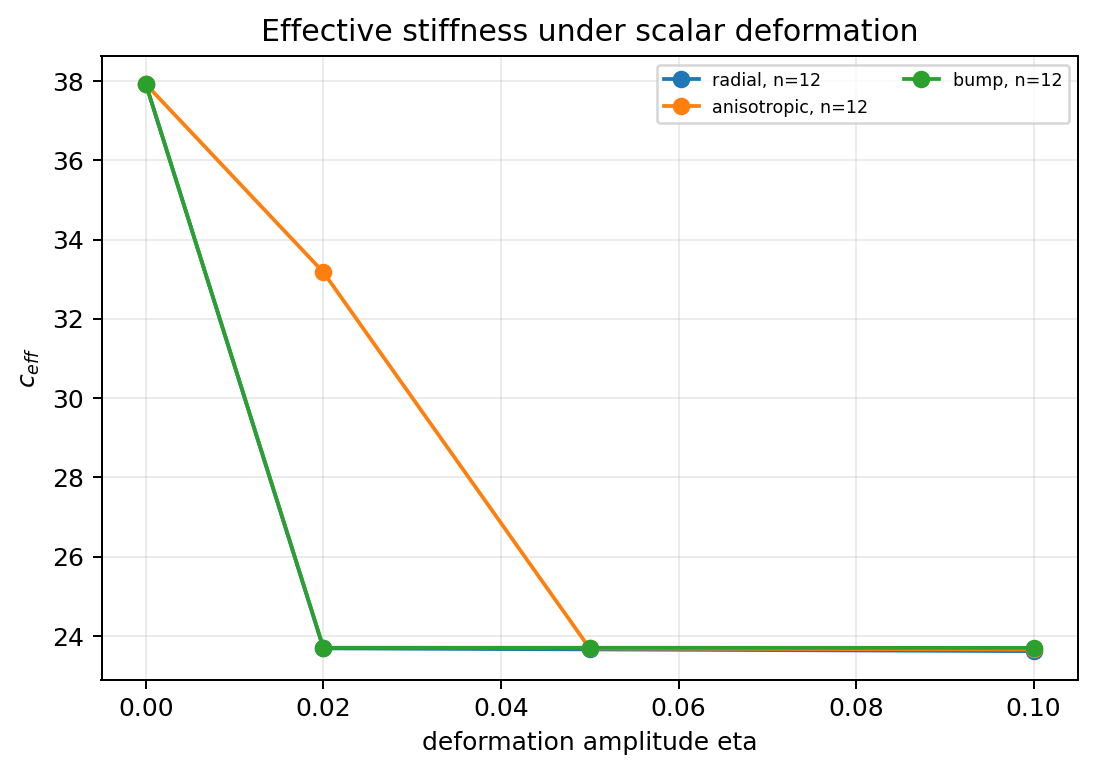
\includegraphics[width=0.48\linewidth]{../plots/20260310_164600_transverse_stiffness_vs_deformation.png}
\caption{Stage 4 effective gap and stiffness response under scalar or kernel-geometry deformation. Left: fitted gap versus deformation amplitude. Right: fitted stiffness versus deformation amplitude.}
\label{fig:gap-stiffness}
\end{figure}

\begin{figure}[t]
\centering
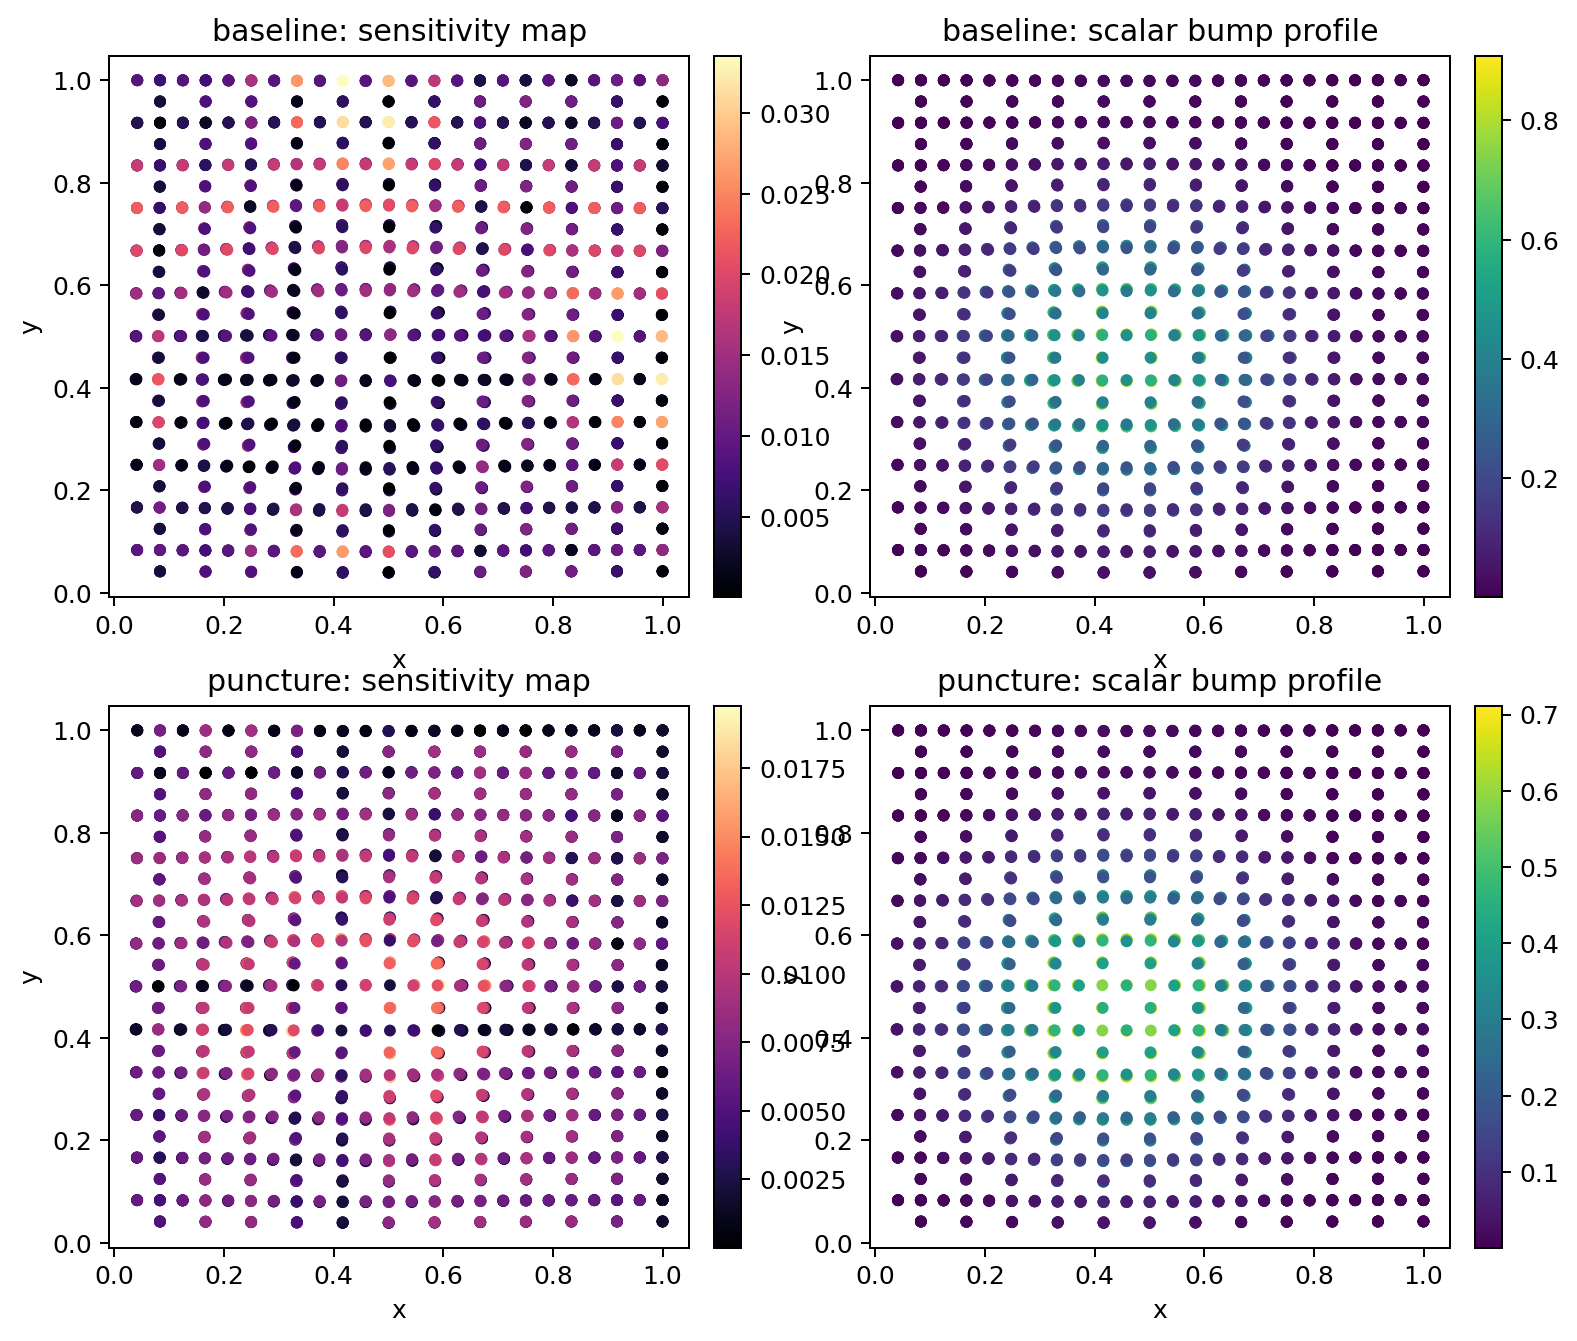
\includegraphics[width=0.48\linewidth]{../plots/20260310_164414_transverse_backreaction_maps.png}
\hfill
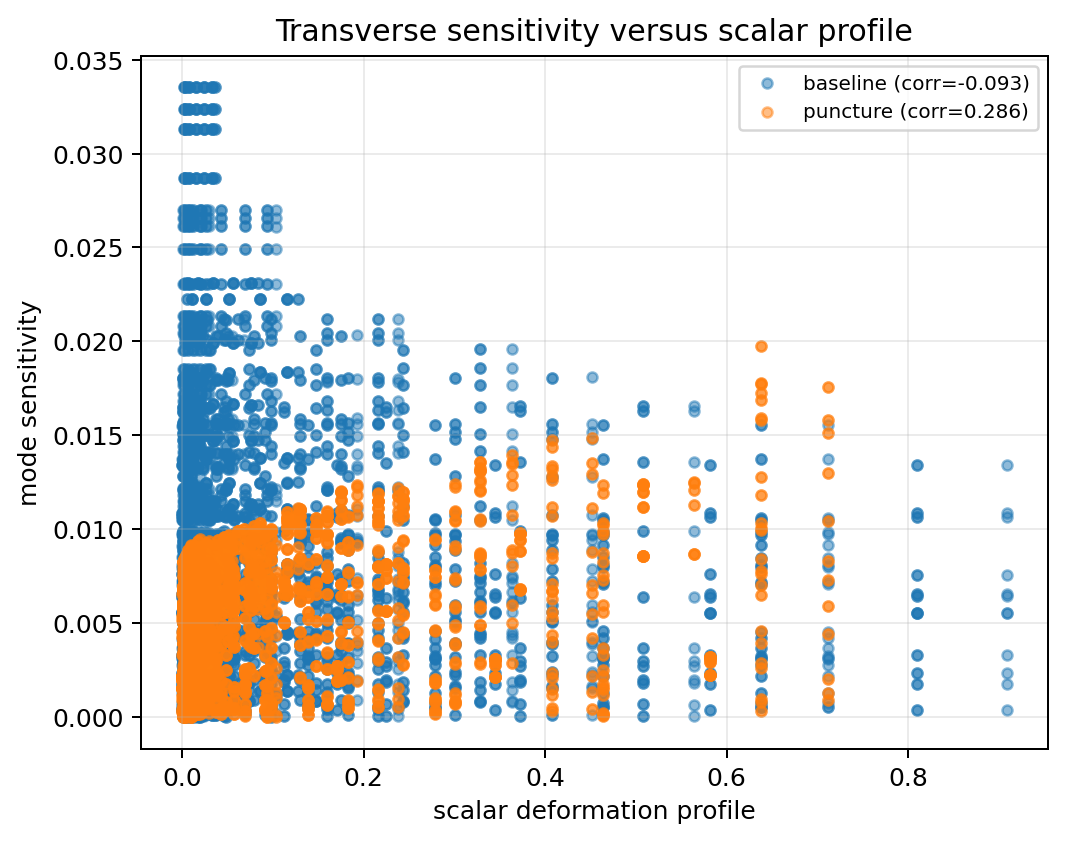
\includegraphics[width=0.48\linewidth]{../plots/20260310_164414_transverse_sensitivity_vs_scalar_profile.png}
\caption{Stage 4 spatial backreaction diagnostics for the localized bump deformation. Left: sensitivity maps for the lowest restricted transverse mode. Right: sensitivity compared with the scalar bump profile.}
\label{fig:backreaction}
\end{figure}

\section{Interpretation Boundary}
The combined Stage 3 and Stage 4 results support a narrow operator-level statement. In the tested range, the restricted transverse band is numerically consistent with a local continuum transverse operator, and smooth scalar or kernel-geometry deformations produce structured spectral response inside that same band. The evidence is carried by spectral ordering, effective low-band fits, real-space correlations, coarse-grained PDE residuals, deformation-induced eigenvalue shifts, coupling matrices, and backreaction maps.

The experiments do not establish Maxwell dynamics, gauge theory, photons, or any particle interpretation. They do not introduce a dynamical gauge field, quantization rule, or continuum interaction law beyond the operator fits already measured. The correct interpretation boundary is therefore the same as in the repository log: this is operator-level numerical evidence only.

\section{Conclusion}
This paper extends the first HAOS-IIP operator preprint without changing the underlying architecture. The frozen Gaussian kernel substrate, scalar branch, edge Hodge operator, and restricted transverse subspace are taken as given, and the new results ask only what continuum operator the transverse band approximates and how that band responds to scalar deformation.

The Stage 3 diagnostics show that the low restricted transverse spectrum is organized like a continuum transverse branch in the tested range. Its low-mode ordering and spacing follow the continuum reference, the effective stiffness is stable near $38$--$39$, the fitted gap remains numerically zero on the clean periodic branch, and the coarse-grained lowest modes satisfy a decreasing-residual curl-curl relation while remaining divergence-free to machine precision. The Stage 4 diagnostics then show that controlled scalar deformations shift this same band in a structured way: stiffness is reduced, a finite gap is opened in the tested deformed fits, low-mode mixing remains organized inside the restricted block, and the backreaction is spatially nonuniform.

The present paper therefore demonstrates operator-level continuum behavior of the restricted transverse sector on the tested kernel substrate together with structured response to scalar deformation. No claim of gauge dynamics or particle interpretation is made. Further work can test denser continuum comparison, larger lattice sizes, and additional operator lifts, including the Stage 5 Dirac-type prototype if that branch is activated.

\section*{Project Resources}
Project website: \url{https://tomislav-rupic.com/}

Code repository: \url{https://github.com/tomislavrupic}

Archived release (Zenodo DOI): \url{https://doi.org/10.5281/zenodo.18938323}

\end{document}
